\begin{boxnote}
      \begin{description}
        \item[種類] Article
        \item[閲覧日] 17th May 2025
        \item[キーワード] Nitrogen Vacancy, Cavity QED
        \item[文献番号] \cite{PhysRevLett.134.183603}
        \item[関連論文] 核スピンを用いた角速度センシング\cite{PhysRevA.86.062104},核スピンと電子スピンを用いた角速度の保存\cite{wang2024spin}
      \end{description}
    \end{boxnote}
    \section{行ったこと}
      \begin{enumerate}
        \item 反転分布なしのメーザをnNV-cQED系で実現.
        \item NVの電子スピン-核スピン-共振器系を用いた,NVを用いた角速度センシングの精度の3桁改善.
        \item 角速度のベクトルセンシング.
        \item 核スピンの環境系によるノイズを影響を電子スピンで補正する共磁力計の実現.
      \end{enumerate}
    \section{詳細}
      \subsection{ドライブ・プローブ干渉}
        NVの電子スピン-核スピン系のハミルトニアンは,
        \begin{align}
          \hat{H}_{\r{NV}} = D\hat{S}^2_z + \gamma_{\r{e}}\hat{\bm{S}}\cdot\bm{B} + Q\hat{I}^2_z - \gamma_{\r{n}}\hat{\bm{I}}\cdot\bm{B} + \hat{\bm{S}}\mathcal{A}\hat{\bm{I}}
        \end{align}
        と書ける.
        ただし,$\hat{S}_z$は電子スピンの演算子,$\hat{I}_z$は核スピンの演算子,$\mathcal{A}$は対角的な超微細構造のテンソルである.
        どちらもスピン1系であり,$\ket{1} \coloneqq \ket{m_{\r{s}} = 0, m_{\r{I}} = -1}$,$\ket{2} \coloneqq \ket{m_{\r{s}} = 0, m_{\r{I}} = 0}$,$\ket{\r{e}} \coloneqq \ket{m_{\r{s}} = 1, m_{\r{I}} = -1}$のような
        \Lambda 型準位として用いる.
        \begin{figure}[H]
          \centering
          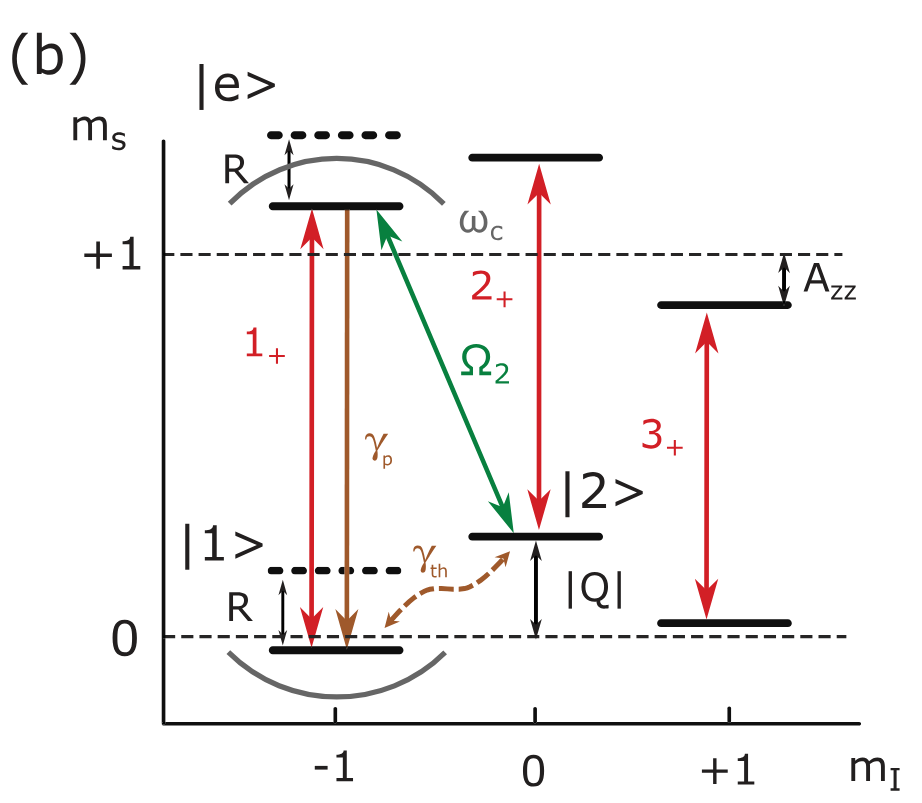
\includegraphics[width = 0.5\linewidth]{/home/hawk/desktop/lab/papers/src/Cavity-Enhanced_Solid-State_Nuclear_Spin_Gyroscope/1_b.png}
          \caption{
            今回用いるNVの準位図.
            横軸が核スピン,縦軸が電子スピンを表している.
          }
        \end{figure}
        $N$個のNVが集まったアンサンブルを考える.
        プローブとして,共振器(マイクロ波)のモード$\hat{a}$は,エネルギー差が$\omega_{\r{c}}$である$\ket{1}$と$\ket{\r{e}}$と結合しているとする
        また$\ket{2}$と$\ket{\r{e}}$を遷移するRabi周波数が$\Omega_2$となるように周波数$\omega_{\r{d}}$のドライブ光が入っているとする.
        共振器の結合$g$が共振器の緩和レート$\kappa$や電子スピンのデコヒーレンスレート$\Gamma$よりも十分大きい,$C = 4g^2 / (\kappa\Gamma) \sim 20$の強結合領域を考える.
        $\omega_{\r{c}}$と$\omega_{\r{d}}$の離調$\Delta$が0になると,電磁誘導透過(EIT)が起こる.
        \begin{figure}[H]
          \centering
          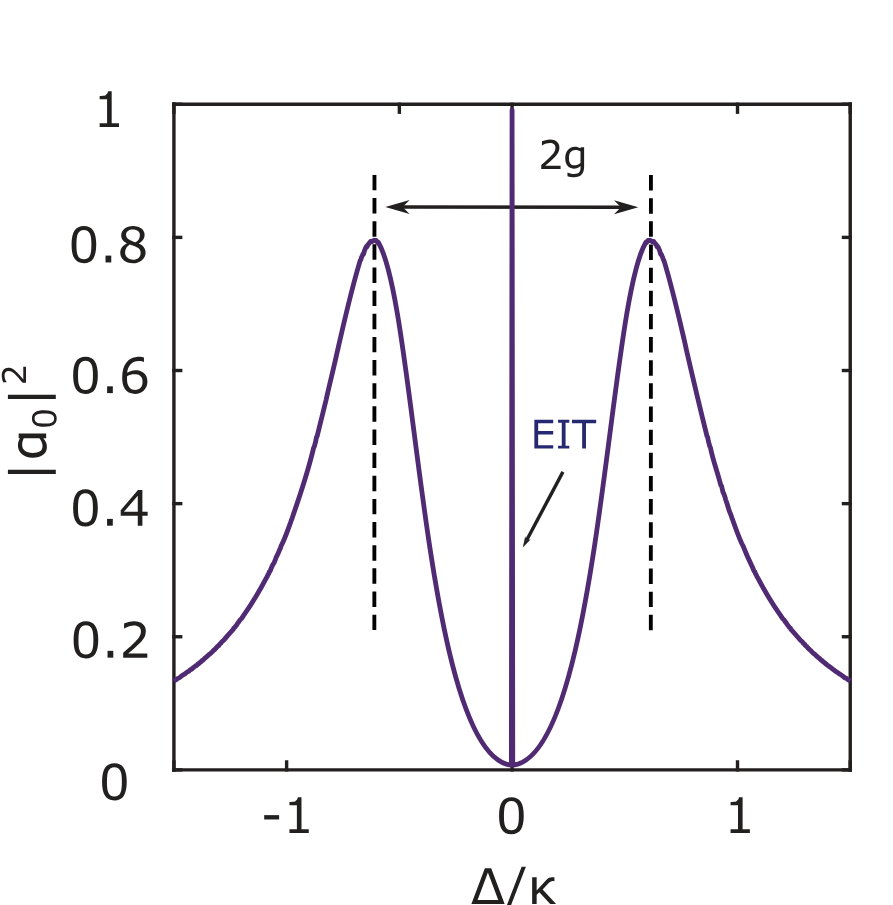
\includegraphics[width = 0.5\linewidth]{/home/hawk/desktop/lab/papers/src/Cavity-Enhanced_Solid-State_Nuclear_Spin_Gyroscope/1_d.png}
          \caption{EITの様子.$\abs{\alpha}_0$がNVセンターの吸収強度を表す.この現象は2つの場の量子干渉ととらえることができる.}
        \end{figure}
        さらにRabi周波数を大きくすると,透過するだけでなく,プローブ光が増強されること(MWI)が分かる.
        \begin{figure}[H]
          \centering
          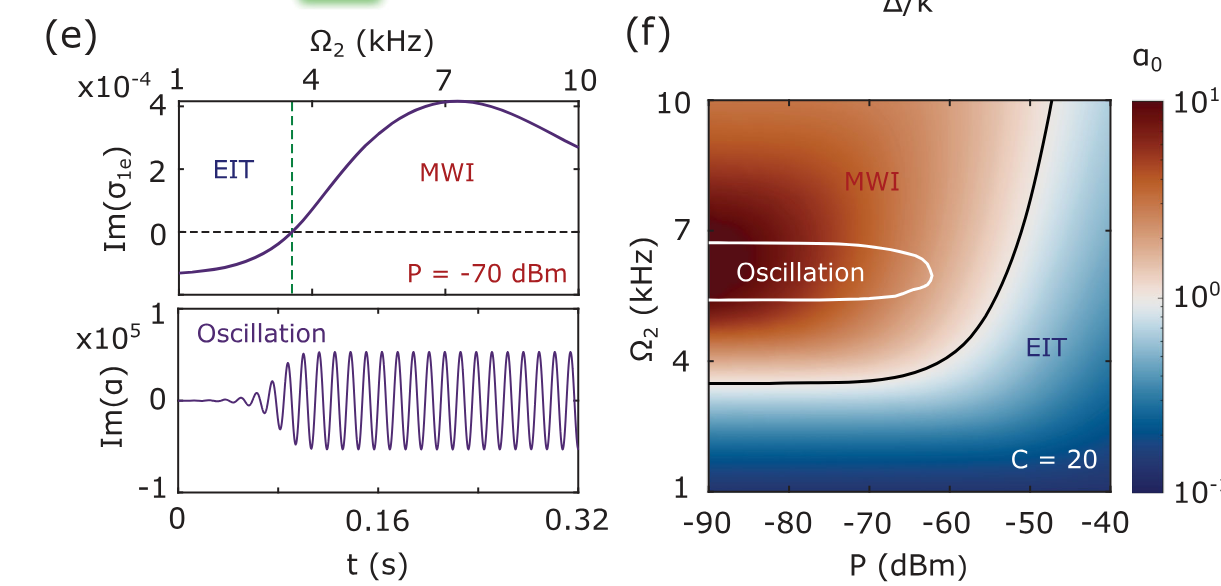
\includegraphics[width = 0.5\linewidth]{/home/hawk/desktop/lab/papers/src/Cavity-Enhanced_Solid-State_Nuclear_Spin_Gyroscope/1_e_d.png}
          \caption{(e): Rabi周波数を大きくするとEITからMWIへと切り替わることがわかる.(f): プローブ光の強度とRabi周波数による,EITとMWIの関係.}
        \end{figure}
      \subsection{角速度センシング}
        角速度$\bm{R}$で回っているとき,ハミルトニアンに$\bm{R}\cdot \hat{I}$の項を足せば良く,エネルギーシフトを意味する.
        この原理を用いると,従来の感度が$\eta_{\r{exp}} = 4.7\ \r{mdeg / s / \sqrt{Hz}}$であったものが,
        MWIの領域では$1.5\ \r{deg / s / \sqrt{Hz}}$,EITの領域では$3.5\ \r{mdeg / s / \sqrt{Hz}}$となる.
        なお,Standard Quantum Limit (SQL)は今回のサンプルの場合,$0.04\ \r{mdeg / s / \sqrt{Hz}}$であり,改善の余地がある一方,ショットノイズ限界からは3桁改善した結果である.
      \subsection{共磁力計による精度改善}
        電子スピンにも同様の原理で測定を行うことで補正を行った.
        \begin{figure}[H]
          \centering
          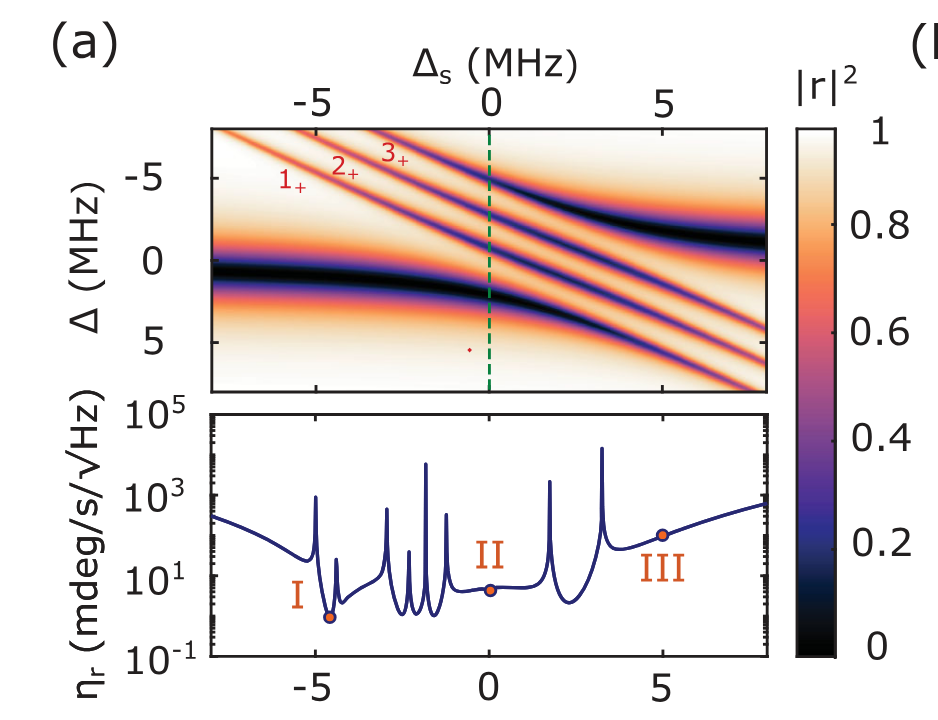
\includegraphics[width = 0.5\linewidth]{/home/hawk/desktop/lab/papers/src/Cavity-Enhanced_Solid-State_Nuclear_Spin_Gyroscope/3_a.png}
          \caption{上: 2つの離調$\Delta$と$\Delta_{\r{s}}$による共振器の透過率$\abs{r}^2$.下: $\Delta_{\r{s}} = 0\ \r{MHz}$としたときの感度.}
        \end{figure}
        $\Delta = -4.7\ \r{MHz}$で感度$\eta_{\r{r}} = 1\ \r{mdeg/s/\sqrt{Hz}}$を達成して,単純な角速度センシングよりも改善していることが分かる.
        実効的には3つ目の核スピンを用いて改善と言っているが,どういうことかよくわからない.